\documentclass[12pt]{article}

\usepackage{natbib}

\usepackage{amssymb}
\usepackage{amsmath}
\usepackage{bm}
\usepackage{dsfont}
\usepackage[margin=1.00in]{geometry}
\usepackage[font=scriptsize]{caption}
\usepackage{dsfont}
\usepackage{amsmath}
\usepackage{graphicx}
\usepackage{bm}
\newcommand{\m}[1]{\mathbf{\bm{#1}}}
\newcommand{\R}{I\hspace{-4.4pt}R}
\newcommand{\bc}[1]{\textcolor{blue}{\mathbf{#1}}}
\newcommand{\ind}{\mathds{1}}

% \setlength\parindent{0pt}

\makeatletter
\setlength{\@fptop}{0pt}
\makeatother

% TODO: should make a reference to Coles somewhere

% TODO: prepare new section for bivariate analysis (references)

\begin{document}

\begin{Large}
\noindent \textbf{Extreme value comparison of CanCM4 simulations and observations}
\end{Large}
\bigskip

%\begin{large}
\noindent Mickey Warner, Bruno Sanso
%end{large}


\bigskip
\bigskip
\begin{quote}
\textbf{Abstract.} Our goal is to explore similarities and differences in extreme behavior between climate simulations and an observation product. We fit a Bayesian hierarchical threshold exceedance model to CanCM4 climate simulation replicates (i.e. simulations having different input settings). Three simulation classes are analyzed: decadal, historical, and pre-industrial control. These are compared against an observation product to which a standard univariate threshold exceedance model is fit. Comparisons are made visually with posterior parameter intervals and numerically using the Bhattacharyya distance between probability densities. We find that in some domains, the simulations are in agreement with the observations, but in others can be quite different.
\end{quote}

\section{Introduction}
\label{intro}

The main focus of this paper is to compare the extreme values of an observation product with those of CanCM4 climate simulations. Specifically, a key question we address is, ``With respect to the extremes, could the observations have come from the climate model?'' The answer to this question would inform us whether the climate model is a reasonable representation of observed extremes.

The Fourth Generation Coupled Global Climate Model (CanCM4) from the Canadian Centre for Climate Modeling and Analysis (CCCma) is made up of an atmospheric component, CanAM4 \citep{von2013canadian}, and an ocean component, CanOM4. The two components are coupled daily to produce climate predictions of a variety of variables on a roughly $2.5^\circ$ degree grid over the globe (see \cite{merryfield2013canadian}). Two variables will be analyzed: precipitation (labled \texttt{pr}, in meters) and maximum temperature (labeled \texttt{tasmax}, in Kelvin). We further restrict our attention to analyzing two seasons---summer and winter---and two regions---California and the U.S.

Three experimental classes that are of particular interest are decadal, historical, and pre-industrial control runs. The decadal simulations provide climate estimates for ten years into the future, after conditioning on the state of the ocean at the time. We consider two decades in this analysis: 1962--1971 and 1990--1999, which are conditioned on ocean states in 1961 and 1989, respectively. Historical simulations are obtained for the years 1961--2005 and are noted for including events that affect the climate such as volcanoes. The pre-industrial control, or simply control, simulations begin at climate conditions comparable to those preceding the industrial revolution and are run over a thousand years. The purpose of the control runs is to provide some measure of internal variability of the climate system. Decadal and historical simulations are run at $R=10$ different input settings. To obtain $R=10$ ``replicates'' for the control simulations, we randomly select ten non-overlapping 10-year periods.

An observation product is obtained from \cite{maurer2002long}. The observations are based on daily measurements from weather stations throughout the United States and are interpolated onto a fine grid (about $1/8^\circ$ degree spacing). To make the observations comparable to the climate simulations, we take weighted sums or averages of the climate simulations and just sums or averages of the observations. See section \ref{process} for details, along with other changes made to the data in preparation for analysis.

The classic approach to analyzing extreme values is to model block maxima (e.g. annual maxima). It can be shown that under certain conditions the block maxima of independent random variables has a distribution which belongs to the generalized extreme value (GEV) family of distributions. Such an approach naturally requires omitting a large portion of the data. This can be remedied by using a threshold exceedance model which involves selecting some large threshold and fitting the exceedances to the generalized Pareto distribution (GPD). We take the threshold exceedance approach in this paper (section \ref{thresh}). See \cite{coles2001introduction} for an excellent introduction to these and other approaches in extreme value analysis.

% Being a threshold exceedance analysis, we must concern ourselves with exceedances occuring together within a short time. This is handled by studying the extremal index $\theta$, a measure of dependence among the extremes. With an estimate for $\theta$, we can ``decluster'' the exceedances to obtain independent clusters. The method for estimating $\theta$ and declustering has been generalized to the hierarchical setting, see section \ref{index}.

% Having replicates of a time-series suggests the use of a hierarchical model, described in detail in section \ref{hier}. Under such a framework we can model each series separately, while assuming these series come from a larger population. In the analysis, we will place focus on the mean of this larger population, being akin to the ensemble average in a climate study.

We attempt to answer the question posed at the beginning of this introduction by comparing posterior intervals for statistical model parameters and other quantities such as return level (section \ref{return}) and Bhattacharyya distance (section \ref{bhatta}).



\section{Data processing}
\label{process}

\subsection{Aggregation}
\label{aggregate}

\begin{figure}
\begin{center}
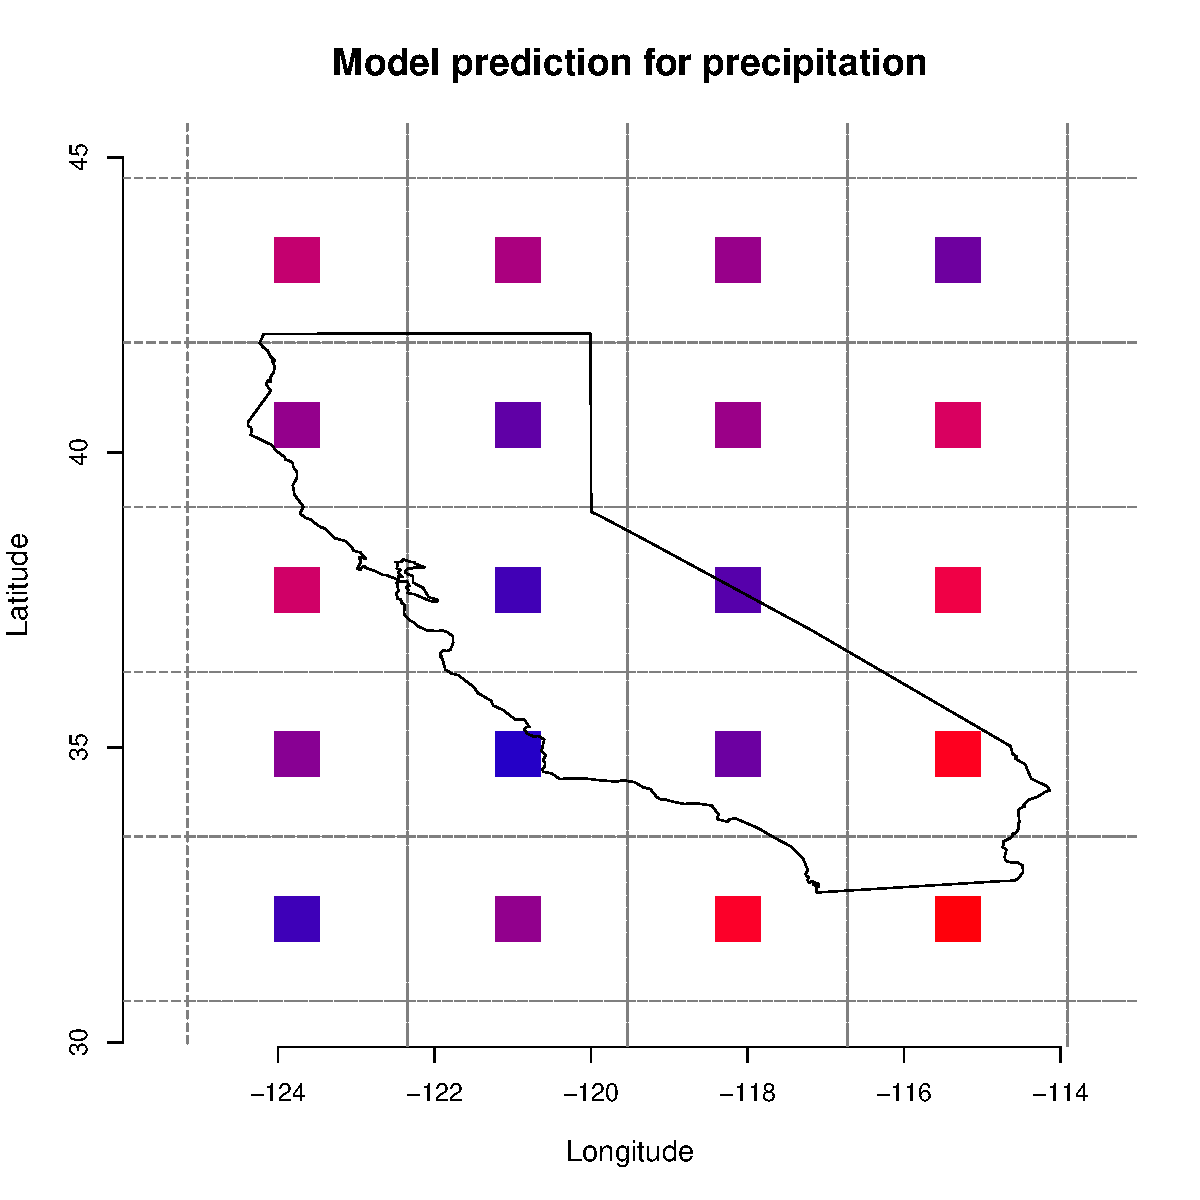
\includegraphics[scale=0.26]{figs/cal_mod_box1.pdf}
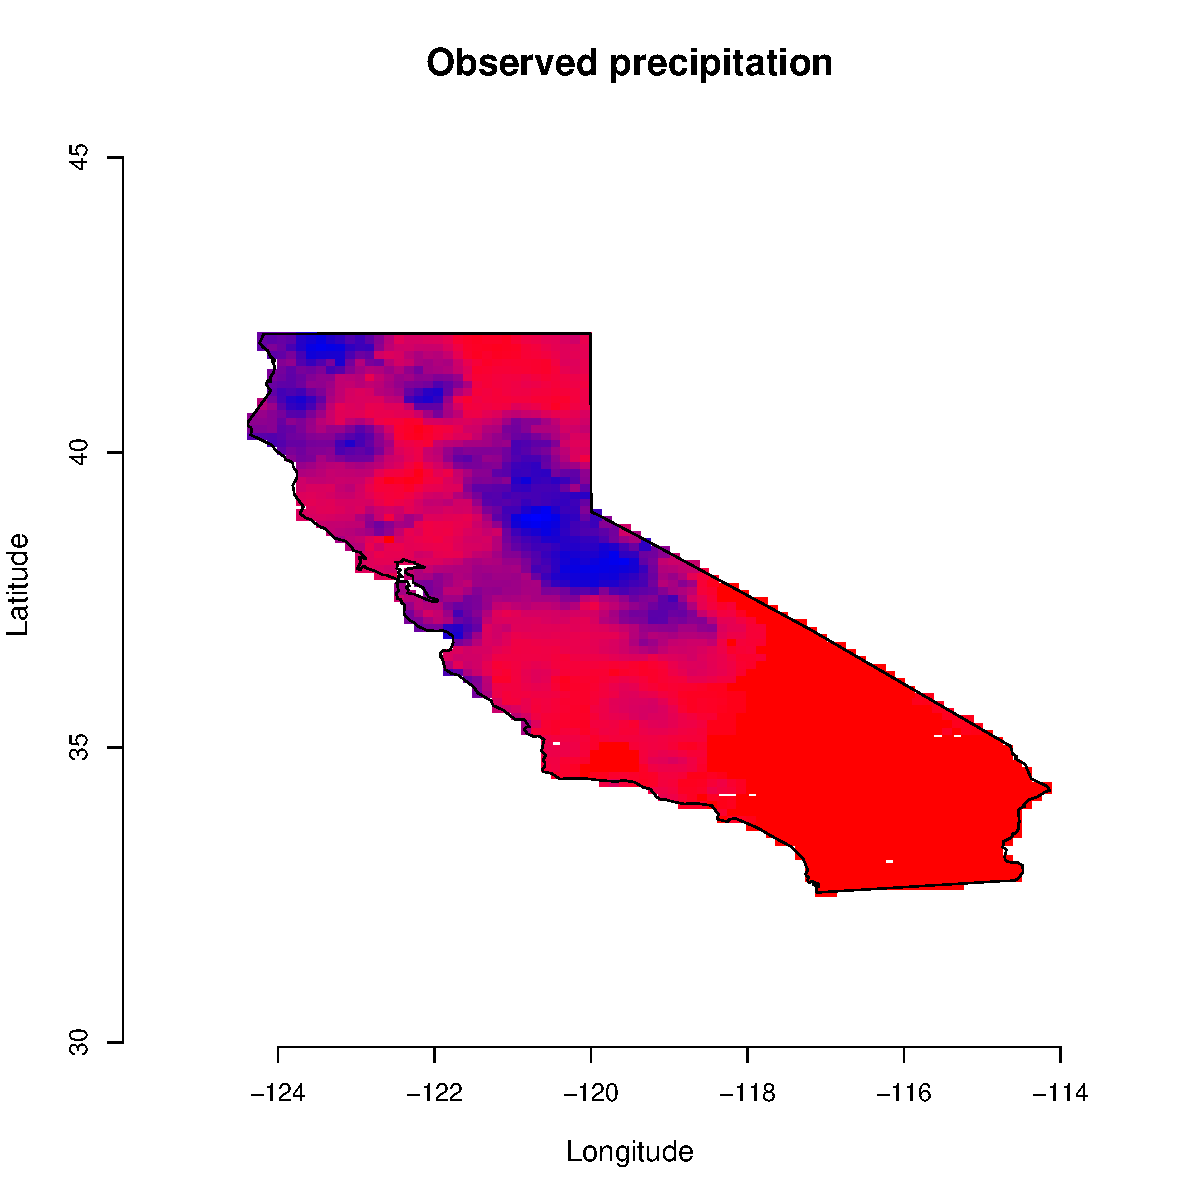
\includegraphics[scale=0.26]{figs/cal_mod_box2.pdf}
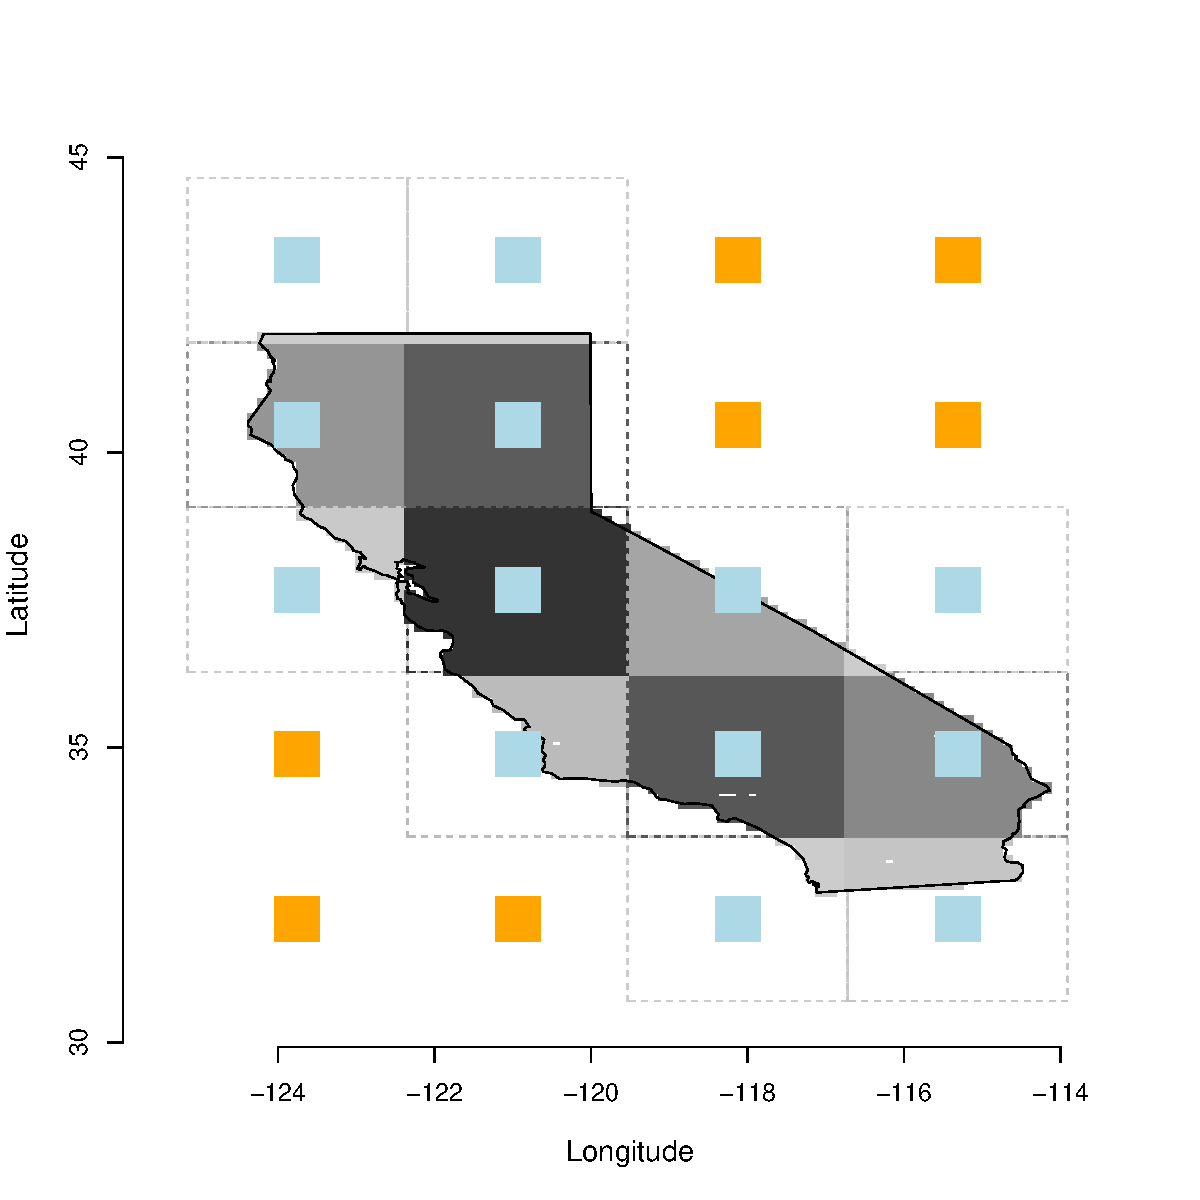
\includegraphics[scale=0.26]{figs/cal_mod_box3.pdf}
\end{center}
\caption{Left: CanCM4 simulation grid cells. Center: Observation locations. Right: method for computing weighted sum or average for CanCM4 to make values comparable with observations; the lighter gray points mean less weight is applied to the climate simulations and the darker gray means more weight. The data shown are from a single day in January.}
\label{weight}
\end{figure}

In this subsection, we describe how the simulations and observations were made to be comparable. Figure \ref{weight} shows the spatial locations of each data source. The plots show only California, but the climate simulations were over the entire globe and the observation product over the United States.

We will analyze precipitation and temperature over both California and the United States. In each case, we take the climate grid cell locations and create non-overlapping cells, or rectangles, such that each location is roughly in the center of the cell. Then we count the number of locations from the observation product that are contained within each cell. The number of locations within the cells are used to weight the climate simulations (the right-most plot in Figure \ref{weight} shows which climate simulation locations have non-zero weight). For precipitation, we take a weighted sum and for temperature a weight average. No weighting is used for the observations. Instead, a straight sum or average of all locations within our region of interest (either California or U.S.) is used. This method places the simulations and the observations on the same scale and yields time-series on daily time scales.

\subsection{De-trending}
\label{anomaly}

\begin{figure}
\begin{center}
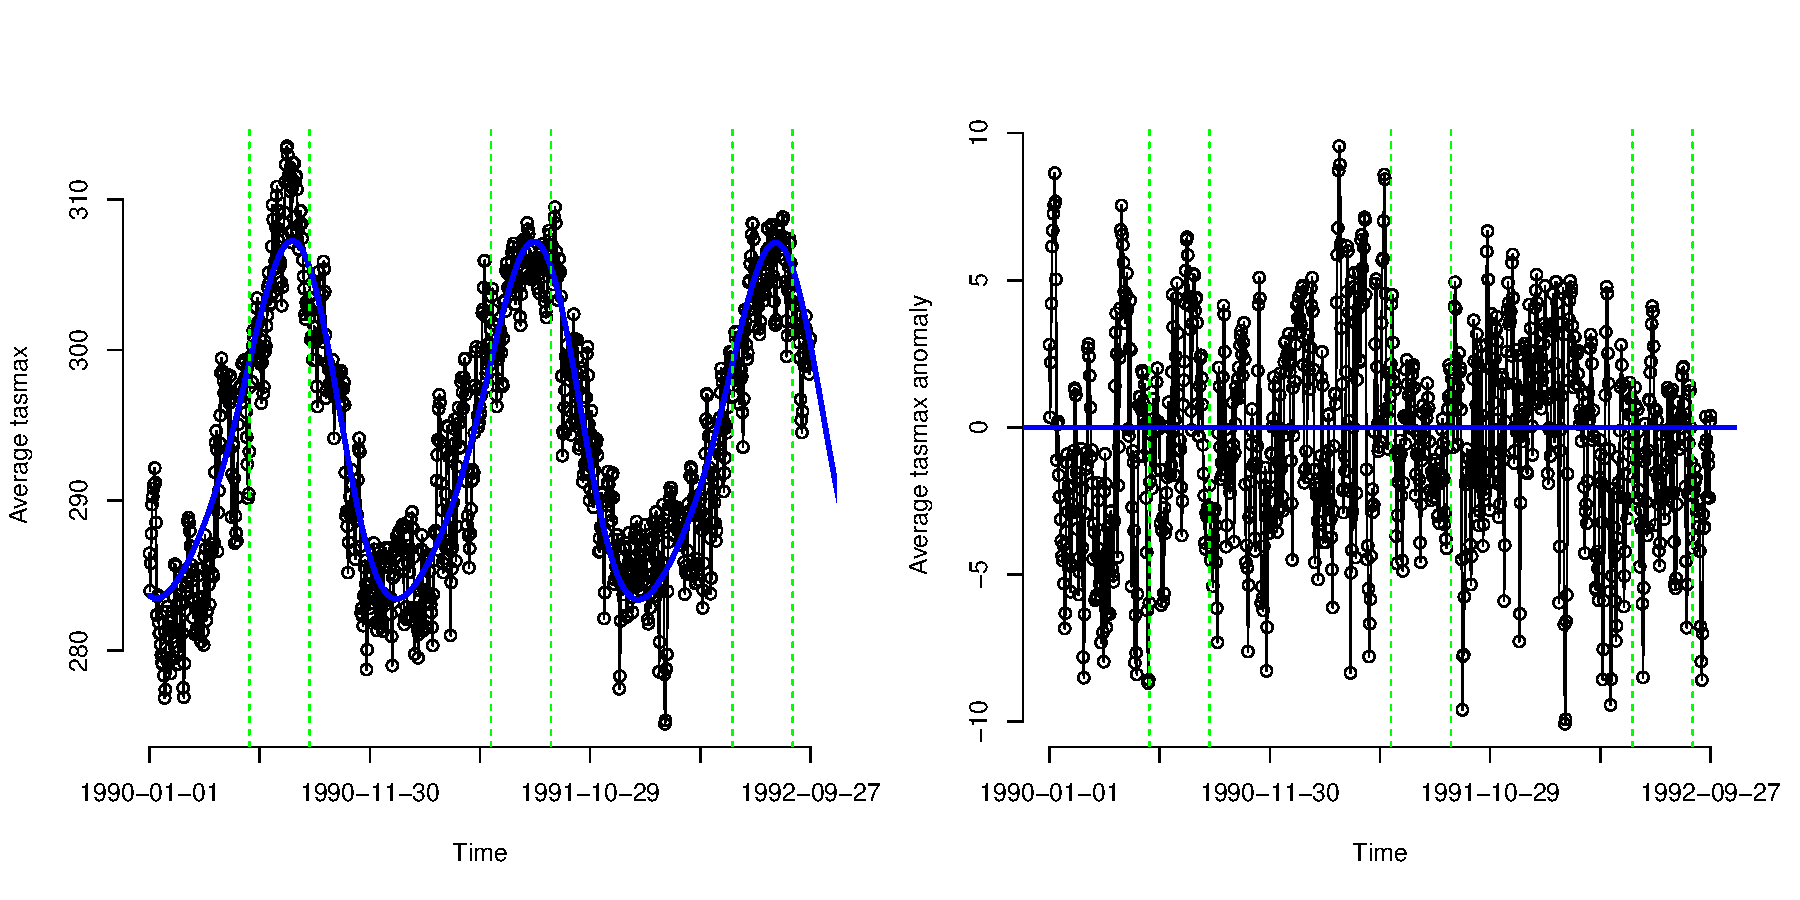
\includegraphics[scale=0.50]{figs/dlm.pdf}
\end{center}
\caption{One of the DLMs used to calculate the anomalies. Shown is one of the decadal replicates of average \texttt{tasmax} in California for about the first two and one-half years of the time-series. The green dashed lines mark the beginning and the end of the summer months.}
\label{dlm_fig}
\end{figure}

Climate data are often non-stationary series characterized by complicated trends and cycles. As such, these present problems when studying extremes. Since we are interested in the behavior of the extremes, each time-series is ``de-trended'' prior to parameter estimation. This is accomplished through the use of dynamic linear models (DLMs). We will review some basic concepts for DLMs, see \cite{prado2010time} chapter 4 for more details.

A normal DLM is specified by the quadruple $\{\m{F}_t, v_t, \m{G}_t, \m{W}_t\}$ which determine how a univariate time series $y_1,\ldots,y_T$ is modeled over time. We assume
\begin{align}
y_t &= \m{F}_t^\top\m{\theta}_t + \nu_t,~~~~~\nu_t\sim N(0, v_t) \label{dlm_model} \\
\m{\theta}_t &= \m{G}_t\m{\theta}_{t-1}+\m{w}_t~~~~~\m{w}_t\sim N(\m{0}, \m{W}_t) \nonumber
\end{align}
where $\m{\theta}_t$ is the length-$p$ state vector, $\m{F}_t$ is a length $p$ vector of known constants are regressors, $\nu_t$ is obersvation noise, $\m{G}_t$ is the known $p\times p$ state evolution matrix, and $\m{w}_t$ is the state evolution noise. Note that $\nu_s$ and $\m{w}_t$ are independent and mutually independent.

An advantage to model (\ref{dlm_model}) is its capability in yielding a smooth and flexible mean across time. After conditioning on the data up to time $T$, we extrapolate back over time to obtain the posterior distributions $p(\m{\theta}_t|D_T)$ for all $t<T$, which have mean $\m{a}_t$. Using these distributions, and given $\m{F}_t$, the mean of $y_t$ is simply $\m{F}_t^\top\m{a}_t$ (we refer the reader to \cite{prado2010time} for the algorithmic details).

We must omit further details in the interest of space. Our DLM is finalized in the following way. We construct $\m{F}_t$ and $\m{G}_t$ such that the evolution of $\m{\theta}_t$ has annual and semi-annual periods, i.e. the first and second harmonics. Higher harmonics did not seem to make significant contributions in modeling the time-series. A discount factor of $\delta=0.9999$ was chosen, signifying low systematic variance. We assume the prior for $v_t$ is an inverse gamma having sensible shape and scale parameters.

In the end, we are left with the residuals. See Figure \ref{dlm_fig}. The blue line in the left plot is the mean of $y_t$, $\m{F}_t^\top\m{a}_t$, given the whole time series. The interior of the vertical green lines mark the summer months. The right plot is the result of subtracting the observation $y_t$ with the mean from the DLM, which produces a roughly stationary sequence. Thus, in our extreme value analysis we fit our model to the residuals, or anomalies.

For each time-series to be analyzed, we fit a DLM having the characteristics described above to obtain the anomalies. When working within a specific season, either winter (December, January, February) or summer (June, July, August), we concatenate across years to form a single time series of seasonal anoamlies. So, for example in winter, 28 February is followed immediately by 1 December.

\section{Methods}

\subsection{Threshold exceedance model}
\label{thresh}

\subsubsection{Univariate}
\label{univariate}

Under some mild assumptions, for random variable $X$ and for large enough $u$, the distribution of $X-u$ (the exceedance), conditional on $X>u$ is approximately
\begin{align}
P(X-u\leq y|X>u) \approx H(y) = 1 - \left(1+\frac{\xi y}{\sigma}\right)^{-1/\xi} \label{gpapprox}
\end{align}
defined on $\{y:y>0~\mathrm{and}~(1+\xi y/\sigma) >0\}$. $H(y)$ is the distribution function for a generalized Pareto random variable with shape paremeter $\xi\in\R$ and scale $\sigma>0$.

Let $X_1,\ldots,X_n$ be a sequence of i.i.d. random variables and $u$ be a high threshold. Define $Y_i=X_i-u$ for $X_i>u$ be the $k$ exceedances. The likelihood of $(\xi,\sigma)$ is derived from (\ref{gpapprox}) as
\begin{align}
L(y_1,\ldots,y_k;\sigma,\xi)=\sigma^{-k}\sum_{i=1}^k\left(1+\frac{\xi y_i}{\sigma}\right)_+^{-1/\xi-1} \label{gplike}
\end{align}
where $z_+=\max(z,0)$. This provides the basis for an extreme value analysis. For example, after declustering, the cluster maxima (which are roughly independent) may be fit using likelihood (\ref{gplike}).

\subsubsection{Hierarchical model}
\label{hier}

Suppose we have $R$ replicates or computer simulations, each with $n_i$ observations, for $i=1,\ldots,R$. Let $X_{ij}$ denote the $j$th observation in replicate $i$. We assume
\[ X_{ij} \sim F_i,~~~~~i=1,\ldots,R,~~~~~j=1,\ldots,n_i \]
and all $X_{ij}$ are mutually conditionally independent. For a fixed $u$ and each $i$, define the following sets:
\[ A_i = \{j:x_{ij}\leq u\},~~~ A_i^c = \{j: x_{ij}>u\} \]
where $|A_i|=n_i-k_i$ and $|A_i^c|=k_i$ with $k_i$ being the number of exceedances in replicate $i$. We define our exceedances as
\[ y_{ij} = (x_{ij}-u)\cdot \ind_{(j \in A_i^c)} \]
so that all observations not exceeding $u$ are marked as $0$. Let $\m{y}_i=(y_{i,1},\ldots,y_{i,n_i})^\top$ and $\m{y}=(\m{y}_1^\top,\ldots,\m{y}_R^\top)^\top$.

The likelihood is given by
\begin{align}
L(\m{y}; \m{\sigma}, \m{\xi}, \m{\zeta}) &= \prod_{i=1}^R f_{Y_i}(\m{y}_i|\sigma_i,\xi_i,\zeta_i) \nonumber \\
&= \prod_{i=1}^R\left[\prod_{j\in A_i} F_{X_i}(u) \times \prod_{j\in A_i^c} f_{X_i}(y_{ij}+u)\right] \nonumber \\
&\approx \prod_{i=1}^R\left[\prod_{j\in A_i} F_{X_i}(u) \times \prod_{j\in A_i^c} [1-F_{X_i}(u)]h(y_{ij}|\sigma_i,\xi_i)\right]~~~~~\mathrm{(approximation~(\ref{gpapprox}))} \nonumber \\
&= \prod_{i=1}^R\left[\prod_{j\in A_i} (1-\zeta_i)\times \prod_{j\in A_i^c} \frac{\zeta_i}{\sigma_i}\left(1+\xi_i\frac{y_{ij}}{\sigma_i}\right)_+^{-1/\xi_i-1}\right]~~~~~(\zeta_i=1-F_{X_i}(u)) \nonumber \\
&= \prod_{i=1}^R\left[(1-\zeta_i)^{n_i-k_i}\zeta_i^{k_i}\prod_{j\in A_i^c}\frac{1}{\sigma_i}\left(1+\xi_i\frac{y_{ij}}{\sigma_i}\right)_+^{-1/\xi_i-1}\right] \label{biglike}
\end{align}

Note that the parameters describing the tail of $F_i$ (i.e. $\xi_i,\sigma_i$) depend only on those observations which exceed $u$. The parameter $\zeta_i=P(X_{ij}>u)$, which is necessary for calculating return levels (section \ref{return}), is based only on the number of exceedances. This justifies the use of cluster maxima for $\m{y}_i$.

We complete the hierarchical model formulation by specifying the following priors:
\begin{align}
\xi_i|\xi, \tau^2  &\sim Normal(\xi, \tau^2) \nonumber \\
\sigma_i|\alpha, \beta &\sim Gamma(\alpha, \beta) \nonumber \\
\zeta_i|\zeta, \eta &\sim Beta(\zeta\eta, (1-\zeta)\eta) \nonumber \\
 \label{priors} \\
\xi &\sim Normal(m, s^2)&  &\tau^2 \sim InvGamma(a_\tau, b_\tau) \nonumber \\
\alpha &\sim Gamma(a_\alpha, b_\alpha)&  &\beta \sim Gamma(a_\beta, b_\beta) \nonumber \\
\zeta &\sim Beta(a_\zeta, b_\zeta)&  &\eta \sim Gamma(a_\eta, b_\eta) \nonumber
\end{align}
By combining (\ref{biglike}) and (\ref{priors}) we obtain the full posterior distribution. Samples are obtained via MCMC.
% TODO: talk about the hyperparameters, latin letters. Some are intending to be a bit informative, like \tau^2 and \zeta, since we have only 10 ``observations'' for the population distributions.


\subsection{Extremal Index}
\label{index}

% Sloppy, may not be technically correct with regard to theta.
The threshold exceedance model described in section \ref{thresh} relies on an assumption of independence which is unrealistic for a time-series. When there is dependence between the random variables, the extremes are related according to the so-called extremal index \citep{leadbetter1983extremes}, denoted by $\theta\in[0,1]$, which arises in the following way, as summarized in \cite{ferro2003inference}. For $\{X_n\}_{n\geq 1}$ a strictly stationary sequence of random variables with marginal distribution $F$, the sequence has extremal index $\theta$ if for each $\tau>0$ there is a sequence $\{u_n\}_{n\geq 1}$ such that,
\begin{align}
\lim_{n\rightarrow\infty} n(1-F(u_n)) &\rightarrow \tau \mathrm{~and~} \nonumber \\
\lim_{n\rightarrow\infty} P(\max(X_1,\ldots,X_n)\leq u_n) &\rightarrow \exp(-\theta\tau). \nonumber
\end{align}
The extremal index describes the behavior of exceedances in the limit and can be loosely interpreted as
\[ \theta = (\mathrm{limiting~mean~cluster~size})^{-1}. \]
As an example, suppose $\theta=0.5$, then we would expect exceedances of a large threshold to occur in pairs; for $\theta=0.33$, in groups of 3.

\cite{ferro2003inference} show that the extremal index arises in the limiting distribution of the times between exceedances of a threshold. If $T_\theta$ is the random variable for interexceedance times in the limit, then $T_\theta$ is distributed according to the mixture
\begin{align}
(1-\theta)\epsilon_0 + \theta \mu_\theta
\end{align}
where $\epsilon_0$ is the degenerate probability distribution at $0$ and $\mu_\theta$ is an exponential distribution with mean $\theta^{-1}$. This means that the role of $\theta$ is two-fold: it is both the proportion of non-zero interexceedance times and the inverse mean of non-zero interexceedance times. This poses a challenge when estimating $\theta$ since is it impossible to observe an interexceedance time of zero in practice.

We next describe the hierarchical model used to esimate $\theta$. This is distinct from the threshold exceedance model and is used only in getting a single estimate for $\theta$, which is used to decluster the exceedances and to calculate return levels.

\subsubsection{Estimation}

Suppose we have observations $X_1,\ldots,X_n$. For a threshold $u$, the $N$ exceedances $Y_i=X_i-u$ given $X_i>u$ occur at times $1\leq j_1<\cdots< j_N\leq n$. The observed interexceedance times are given by $T_i=j_{i+1}-j_i$ for $i=1,\ldots,N-1$. \cite{ferro2003inference} provide the following log-likelihood
\begin{align}
l(\theta, p; \m{T}) =&~ m_1\log(1-\theta p^\theta) + (N-1-m_1)\{\log(\theta)+ \log(1-p^\theta)\} \nonumber \\
 &+ \theta\log(p)\sum_{i=1}^{N-1}(T_i-1) \label{ferro}
\end{align}
where $p$ is the probability of not exceeding the threshold. We require that this likelihood be used in a hierarchical model.

Suppose we have $R$ replicates from a climate model with values from replicate $i$ denoted $X_{i,1},\ldots,X_{i,n}$. If we assume these simulations are independent from each other, then we expect there to be $R$ unique extremal indices $\theta_1,\ldots,\theta_R$. However, since these all come from the same climate model, we may wish to assume that the $\theta_i$ come from a common distribution,
\[ \theta_i \overset{iid}\sim Beta\left(\theta\nu, (1-\theta)\nu\right), \]
having mean $\theta\nu /(\theta\nu + (1-\theta)\nu) = \theta$. Under model (\ref{ferro}), we place a similar prior on the $p_i$,
\[ p_i \overset{iid}\sim Beta\left(p\tau, (1-p)\tau\right). \]

The model is completed by choosing priors for $\theta$, $\nu$, $p$, and $\tau$---the latter two parameters being required only for model (\ref{ferro}). We assume
\begin{align*}
\theta &\sim Beta(a_\theta, b_\theta) \\
\nu &\sim Gamma(a_\nu, b_\nu) \\
p &\sim Beta(a_p, b_p) \\
\tau &\sim Gamma(a_\tau, b_\tau) 
\end{align*}
with the hyperparameters chosen to be
%\begin{table}[h]
\begin{center}
\begin{tabular}{rlcl}
$\theta$: & $a_\theta = 1          $ &~~& $b_\theta = 1/2             $ \\
$   \nu$: & $   a_\nu = 1          $ &~~& $   b_\nu = 1/10            $ \\
$     p$: & $     a_p = 100 \hat{F}$ &~~& $     b_p = 100 (1-\hat{F}) $ \\
$  \tau$: & $  a_\tau = 1          $ &~~& $  b_\tau = 1/10            $ \\
\end{tabular}
\end{center}
%\end{table}
where $\hat{F}=\sum_{i=1}^R\sum_{j=1}^n \ind(X_{i,j}\leq u)$. Our parametrization for the gamma random variables are such that $X\sim Gamma(\alpha,\beta)$ has mean $\alpha/\beta$. The prior values for $\theta$ attempt to mitigate some of the issues surrounding model (\ref{ferro})

By assuming conditional indepedence between the simulations, we can construct the following log-likelihood
\begin{align}
L = \sum_{i=1}^R l(\theta_i, p_i; \m{T}^{(i)}) \label{hiertheta}
\end{align}
where $\m{T}^{(i)}$ is the vector of interexceedance times for replicate $i$ having length $N_i$. In the univariate setting for the observation product, only model (\ref{ferro}) is needed.

\cite{suveges2007likelihood} proposed on an alternative likelihood for estimating the extremal index which dealt with some of the issues noted in \cite{ferro2003inference}. This likelihood was extended in \cite{suveges2010model}. Though there are advantages to the alternative likelihood, we prefer to use that given in (\ref{ferro}). In a separate simulation study, both likelihoods performed very similarly, with some preference to model (\ref{ferro}), within the hierarchical setting.

\subsubsection{Declustering}

Declustering is done as given in \cite{ferro2003inference}. Each replicate is declustered separately. Let $\hat{\theta_i}$ be the posterior mean of the extremal index of each replicate. Calculate $C_i=\lfloor \hat{\theta_i} N_i \rfloor + 1$, the estimated number of independent clusters. Let $T_{C_i}$ be the $C_i$th largest interexceedance time in $\m{T}^{(i)}$. In the case of ties, decrement $C_i$ by one until $T_{C_i+1}$ is strictly greater than $T_{C_i}$. Clusters are formed by grouping the exceedances that are separated in time by no more than $T_{C_i}$. In other words, two exceedances are in the same cluster if their interexceedance time is less than or equal to $T_{C_i}$.

The $C_i$ clusters that will be formed using the above scheme are assumed to be independent. For each cluster we compute the cluster maximum, this being the ultimate quantity used in our inference.

\subsection{Return levels}
\label{return}

A most useful quantity in an extreme value analysis is the return level. Generally, for a distribution $G$, the return level $x_m$ is the solution to
\begin{align}
G(x_m) = 1-\frac{1}{m}
\end{align}
and has the convenient interpretation as the quantity that is exceeded on average once every $m$ observations.
% TODO: needs more intuition

When working with the generalized Pareto model (\ref{gpapprox}), it can be shown that the $m$-observation return level is
\begin{align}
x_m = u +\frac{\sigma}{\xi}\left[\left(m\zeta\theta\right)^\xi-1\right] \label{rl}
\end{align}
where the terms $\zeta$ and $\theta$ account for the probability of exceeding $u$ and being within a cluster, respectively. We can obtain a distribution for $x_m$ using MCMC samples for $(\xi, \sigma, \zeta)$. Posterior samples for $\theta$ are obtained separately from $(\xi, \sigma, \zeta)$, and so we choose to use the posterior mean for $\theta$ when computing return levels. The intention here is avoid possible complications due to the fact we do not have samples of the joint vector $(\xi, \sigma, \zeta, \theta)$.


\subsection{Bhattacharyya distance}
\label{bhatta}

Since our focus is on comparing the climate model simulations with the observations, we must to assess differences between a variety of posterior distributions. A naive approach may be to simply determine whether posterior intervals overlap. Though we make use of visuals in our comparison, we desire a more quantitative approach. Here, we make use of Bhattacharyya distance.

\cite{bhattacharyya1943measure} proposed a means for measuring the degree of similarity between two probability distributions. For two continuous random variables on support $\mathcal{X}$ with densities $p$ and $q$, the Bhattacharyya coefficient is defined as
\begin{align}
BC(p,q)=\int_\mathcal{X} \sqrt{p(x)q(x)} dx \label{bhattacoef}
\end{align}
and the Bhattacharyya distance is 
\begin{align}
D_B(p,q)=-\log BC(p,q).
\end{align}
We use kernel density estimation to calculate $p$ and $q$ along a grid of the support and then approximate the integral in (\ref{bhattacoef}). If the support is different for the two random variables (as will typically be the case when comparing random variables whose parameters determine the support such as the generalized Pareto), we will integrate over the intersection of the supports.

Our approach is to compute distances from the replicates to their mean and determine whether the observations could have reasonably come from the climate model. Taking the shape parameter as an example, from the hierarchical model in \ref{hier} we have posterior samples for $\xi_1^c,\ldots,\xi_R^c$ for, say, some decadal simulations. We also have posterior samples for the mean $\xi^c$. Using the kernel density estimation mentioned earlier, we obtain $R$ Monte Carlo estimates $D_B(\xi_i^c, \xi^c)$, for $i=1,\ldots,R$. From the univariate model \ref{univariate} we have the shape parameter $\xi^o$ for the observation product. Finally, we calculate $D_B(\xi^o, \xi^c)$ and ask whether this quantity falls within the range of $D_B(\xi_i^c, \xi^c)$. When this occurs, we say $\xi^o$ is ``similar'' to the $\xi_i^c$ since the observation differs from the mean climate model in a similar way as the replicates differ from the mean.

\section{Results}
\label{results}

For each of the four data sources (i.e. the three climate simulation classes and the observation produce), there are four factors with two levels each. The factors, with their levels, are:
\begin{enumerate}
\item Variable --- precipitation or maximum temperature
\item Season --- winter or summer
\item Decade --- 1962--1971 or 1990--1999
\item Region --- California or U.S.A.
\end{enumerate}
There are then 16 combinations of the factors to be made. For each combination, the hierarchial model described in section \ref{hier} is fit to the decadal, historical, and control runs; the univariate model in section \ref{univariate} is fit to the observation product since this data source does not have replicates.

Thresholds are chosen to be the $0.95$ quantile for the climate simulations and $0.85$ for the observations. These quantiles were found to be quite reasonable for this data while still giving us enough data with which to fit the models. The values of the thresholds themselves are not too important since different thresholds may produce similar return levels.

\begin{figure}
\begin{center}
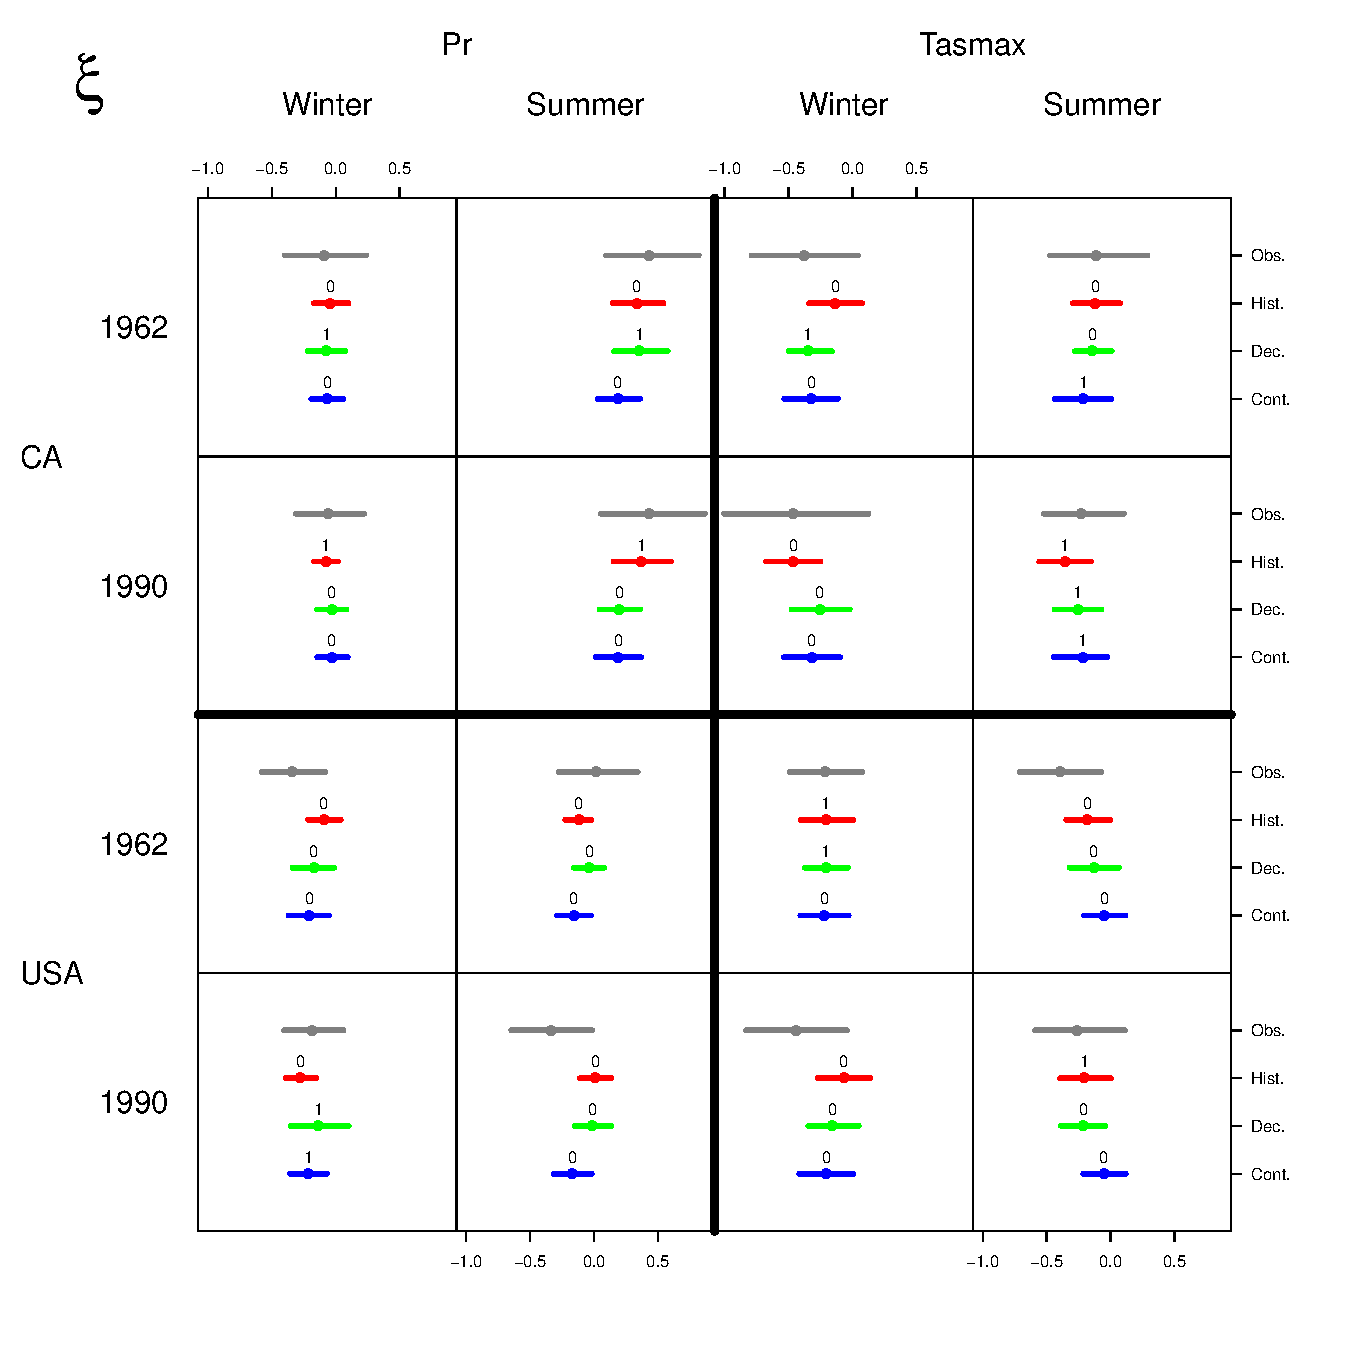
\includegraphics[scale=0.72]{figs/shape.pdf}
\end{center}
\caption{Posterior shape parameter, $\xi$, under each domain and each of the four data types. The points are the means and the lines mark the 95\% h.p.d. intervals. The number above each point marks whether the observations are similar (in the sense of Bhattacharyya distance) to the replicates of that climate model type---1 means similar, 0 mean not similar. Note: The $x$-axes are the same for every plot. The $y$-axes (for this and all subsequent figures) denote only the data type and thus hold no quantitative meaning.}
\label{ksi}
\end{figure}

\begin{figure}
\begin{center}
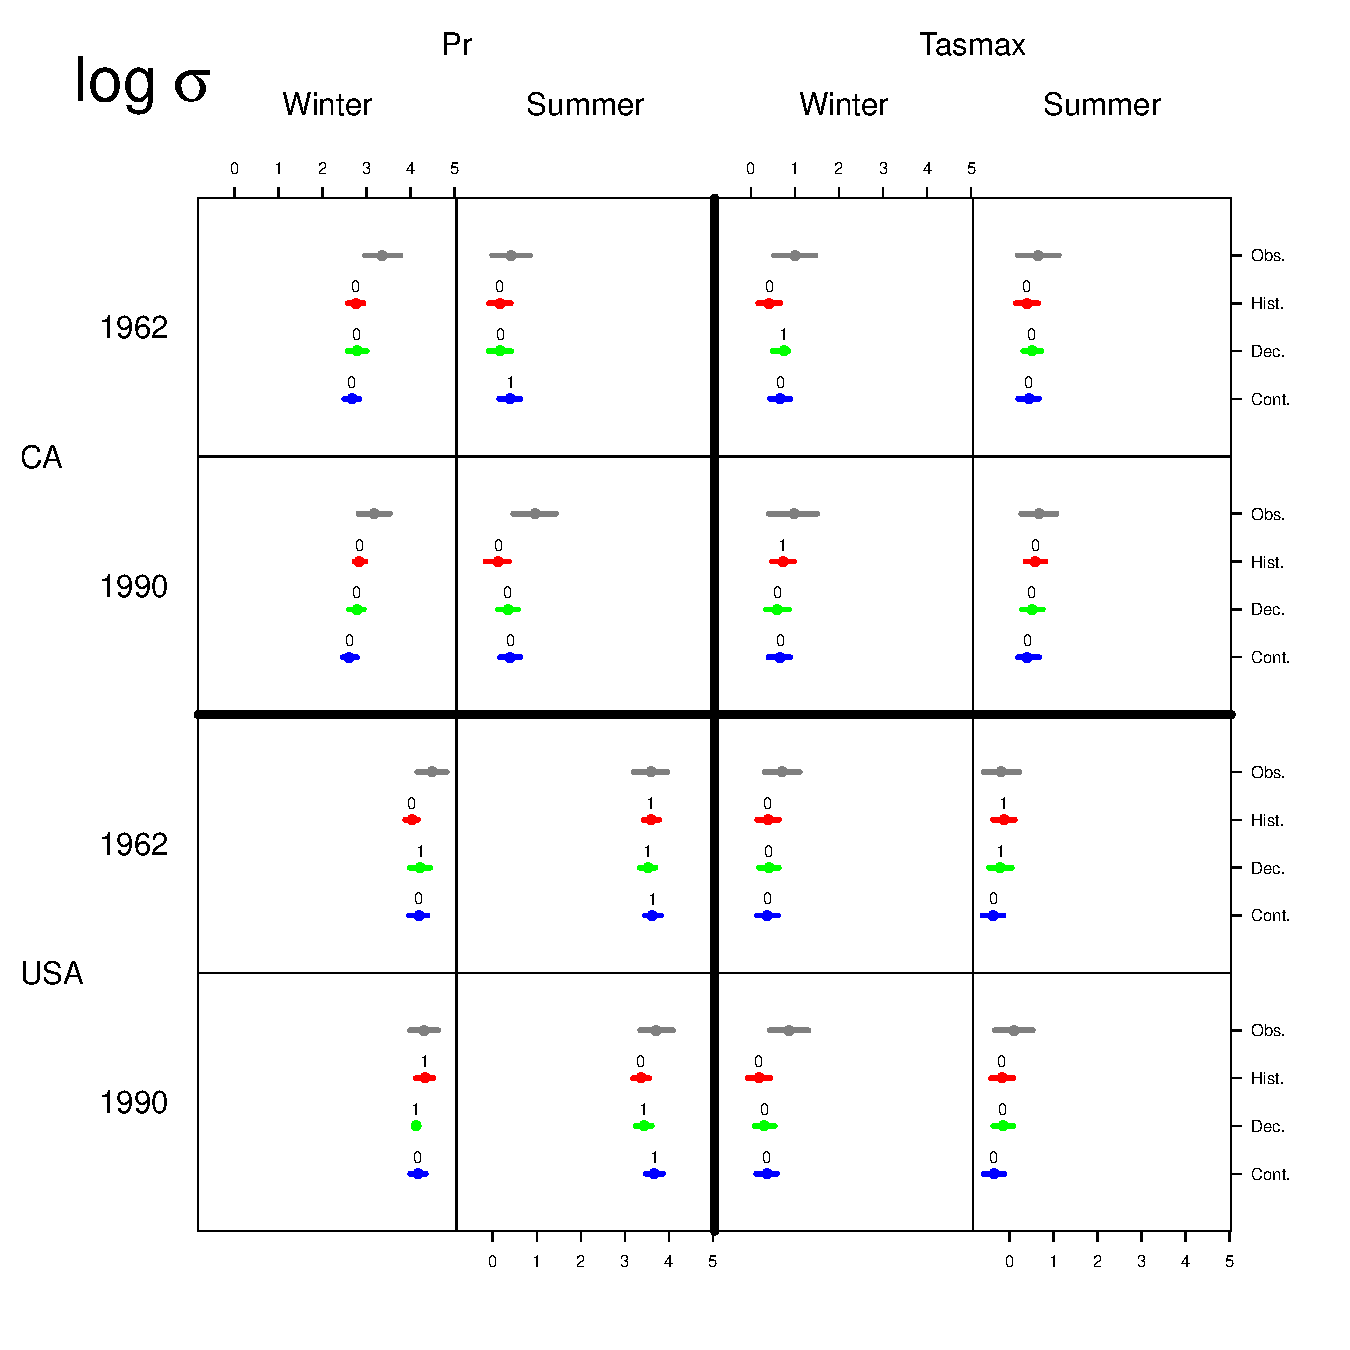
\includegraphics[scale=0.72]{figs/log_sigma.pdf}
\end{center}
\caption{Natural logarithm of the posterior scale. For the CanCM4 simulations, the parameter shown is $\log (\alpha/\beta)$ (the mean scale) because $\sigma_i$ follows a Gamma distribution with mean $\alpha/\beta$. No change of variables is necessary for the observations. Note: The $x$-axes are the same for every plot.}
\label{sigma}
\end{figure}

\begin{figure}
\begin{center}
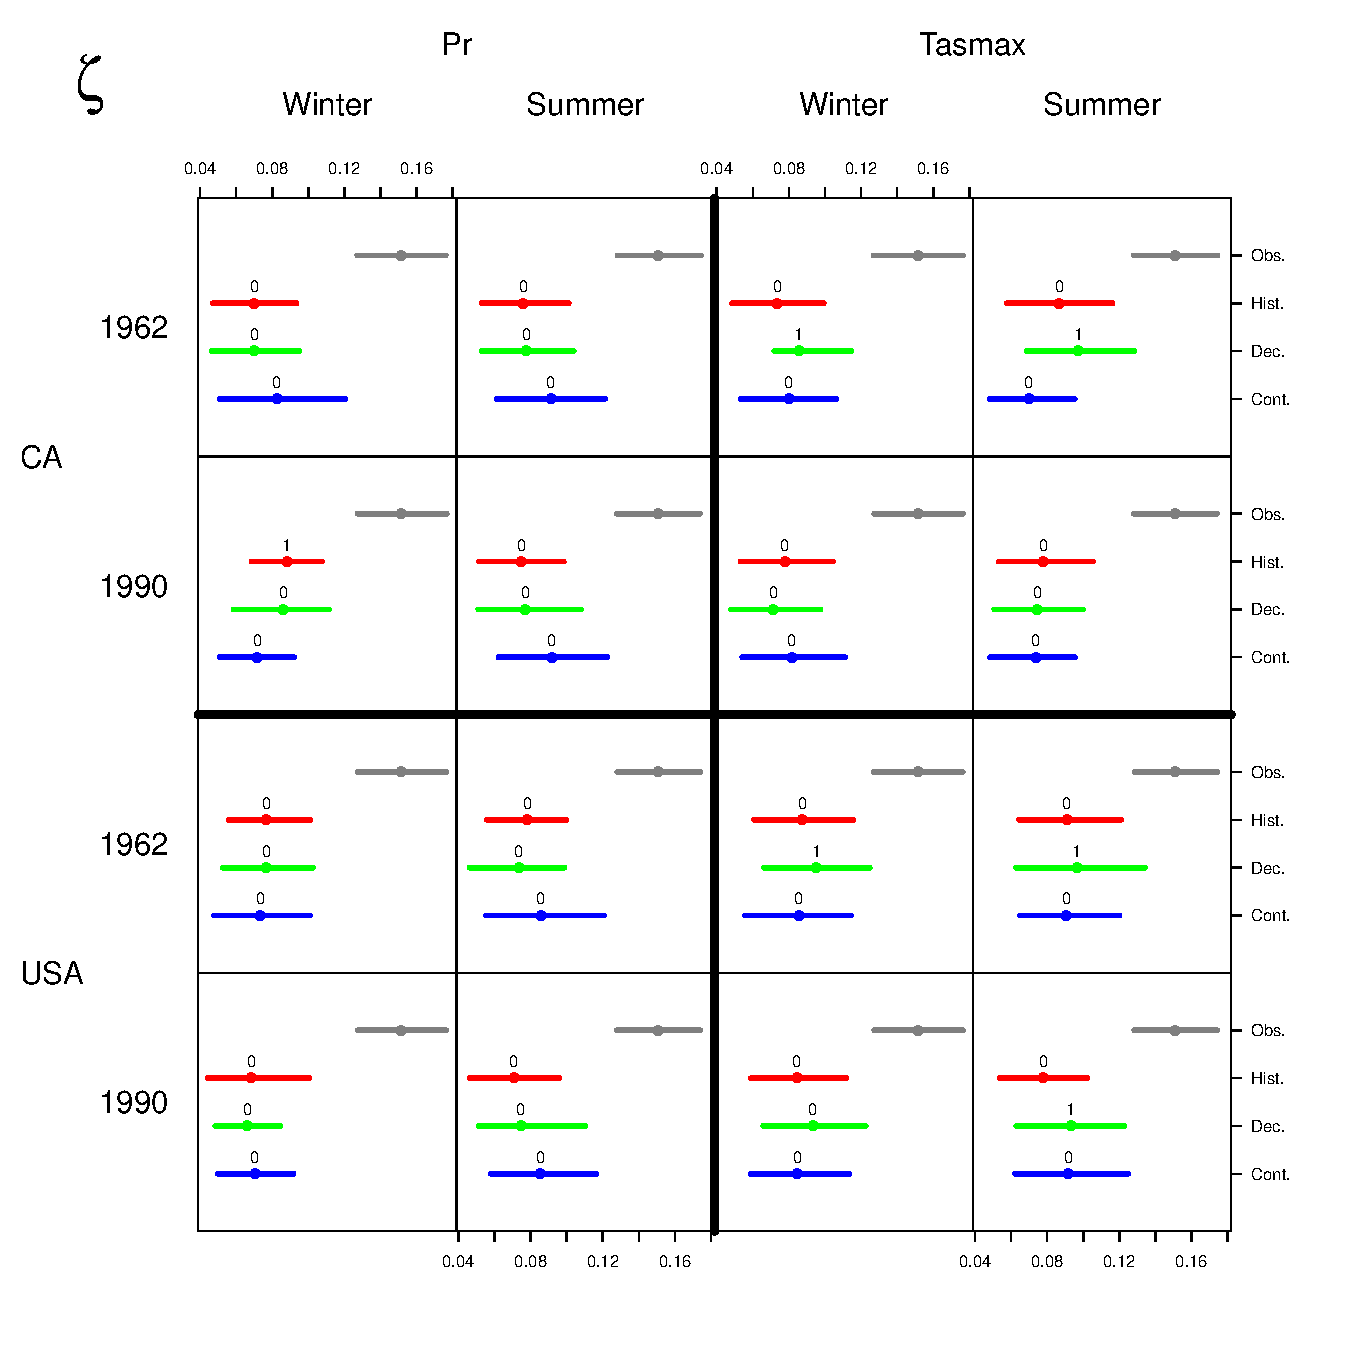
\includegraphics[scale=0.72]{figs/zeta.pdf}
\end{center}
\caption{The probability of exceeding the threshold. These parameters are closely tied to the threshold, a user-specified quantity. Since we chose thresholds as the $0.95$ quantile for the climate simulations and the $0.85$ quantile for the observations, we do not expect there to be much overlap between these posteriors.}
\label{zeta}
\end{figure}

\begin{figure}
\begin{center}
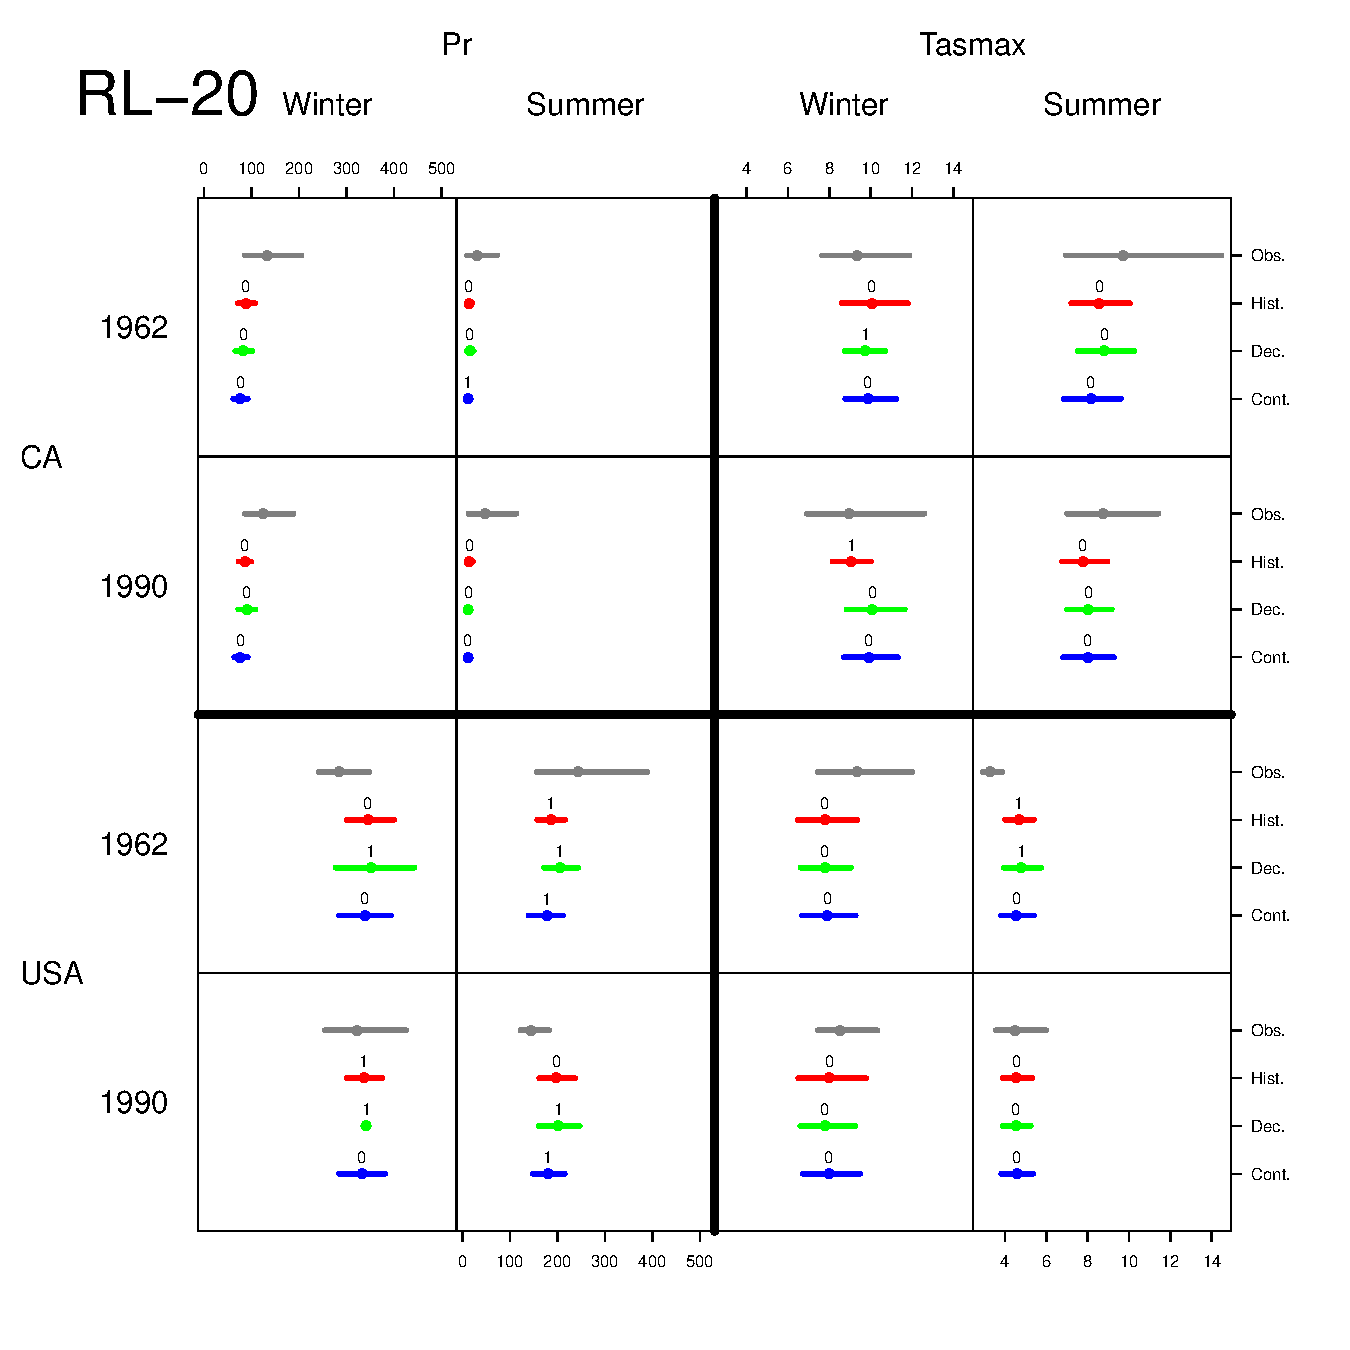
\includegraphics[scale=0.72]{figs/rl20.pdf}
\end{center}
\caption{20-year return levels. Note: The left two columns have the same $x$-axes, which are different than those in the right two columns, which have the same.}
\label{20rl}
\end{figure}

\begin{figure}
\begin{center}
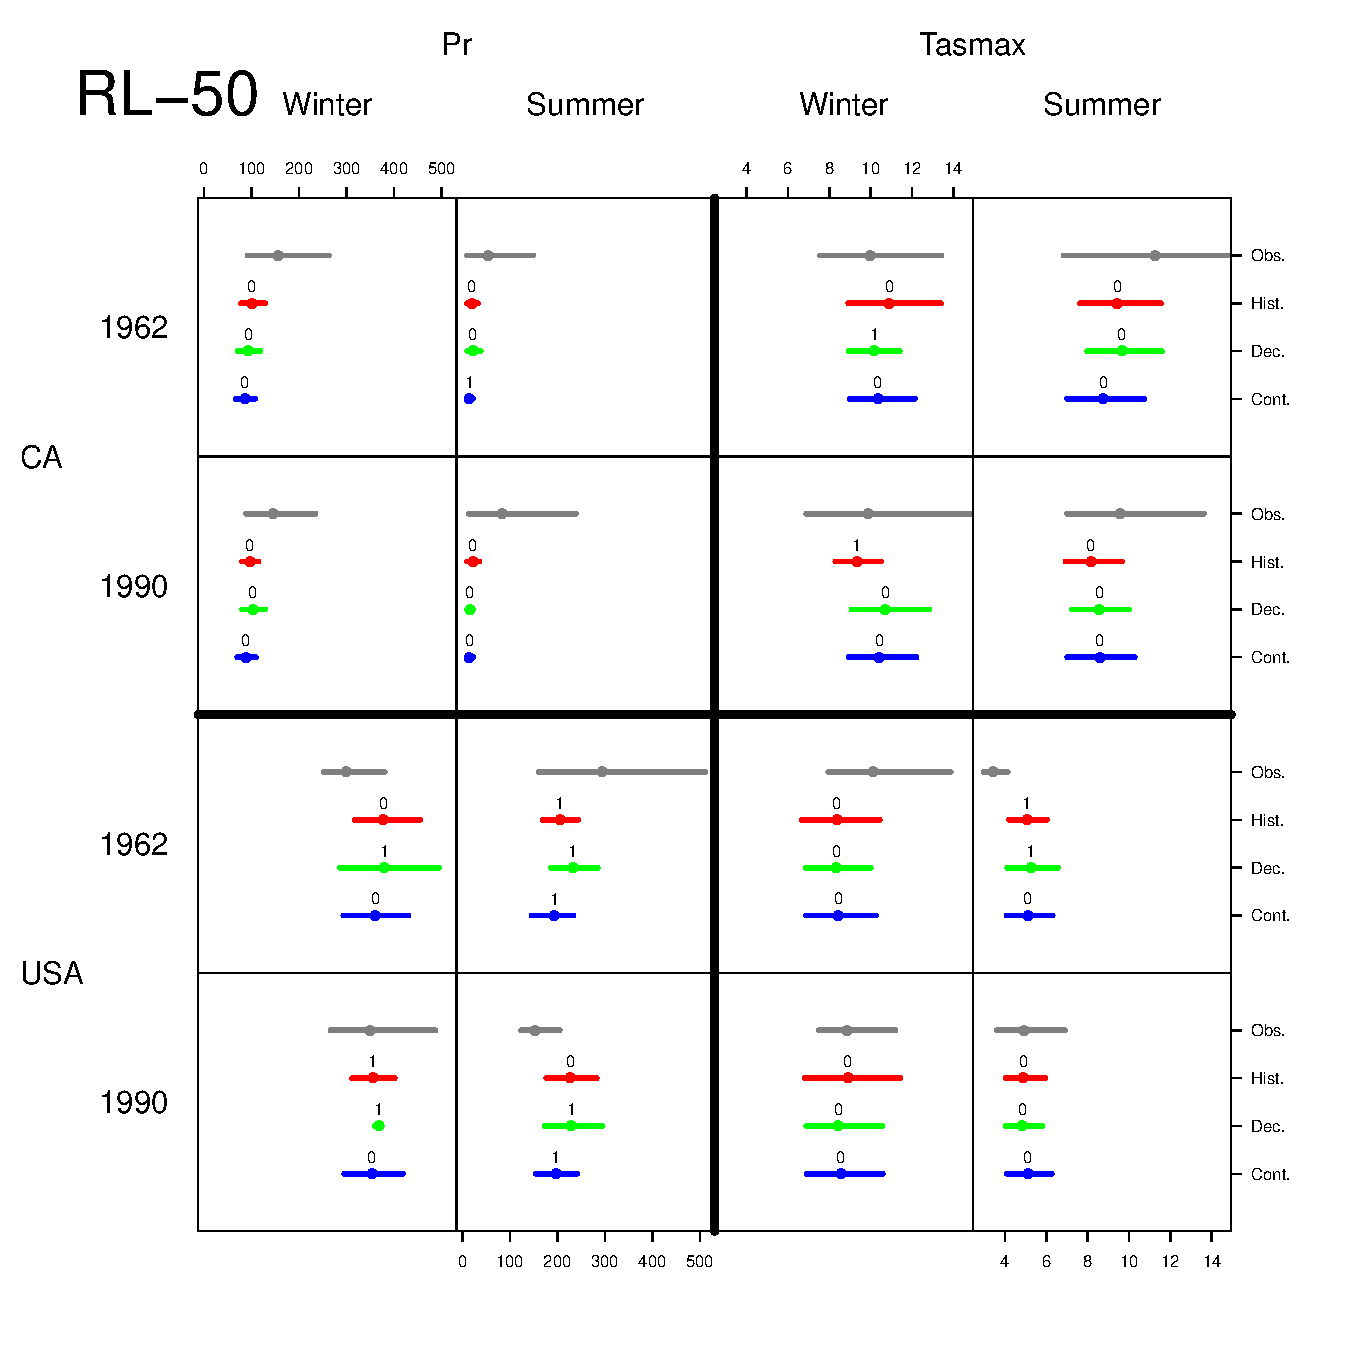
\includegraphics[scale=0.72]{figs/rl50.pdf}
\end{center}
\caption{50-year return levels. The $x$-axes are the same as those in Figure \ref{20rl}.}
\label{50rl}
\end{figure}

\begin{figure}
\begin{center}
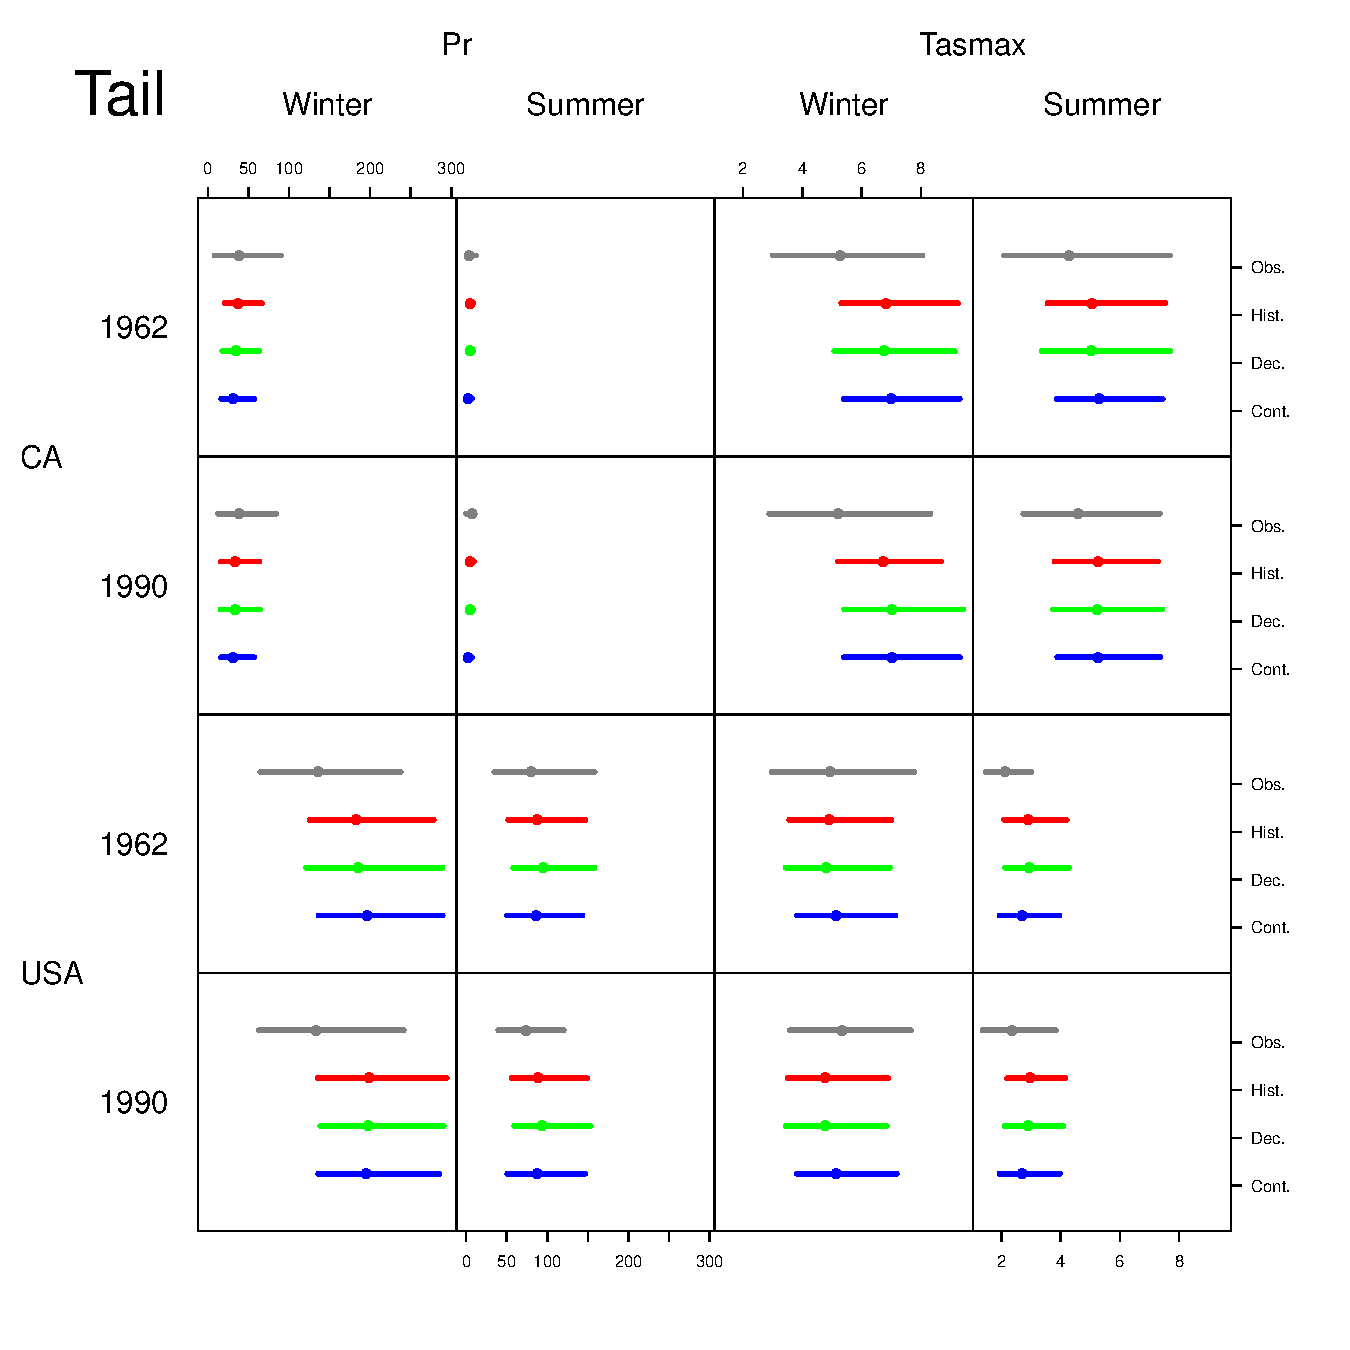
\includegraphics[scale=0.72]{figs/tail.pdf}
\end{center}
\caption{Mean and 95\% h.p.d. for the upper tail (i.e. the generalized Pareto) of the ensemble average. As in Figures \ref{20rl} and \ref{50rl}, the left two columns have the same $x$-axes and the right two columns have the same $x$-axes.}
\label{tail}
\end{figure}

\begin{figure}
\begin{center}
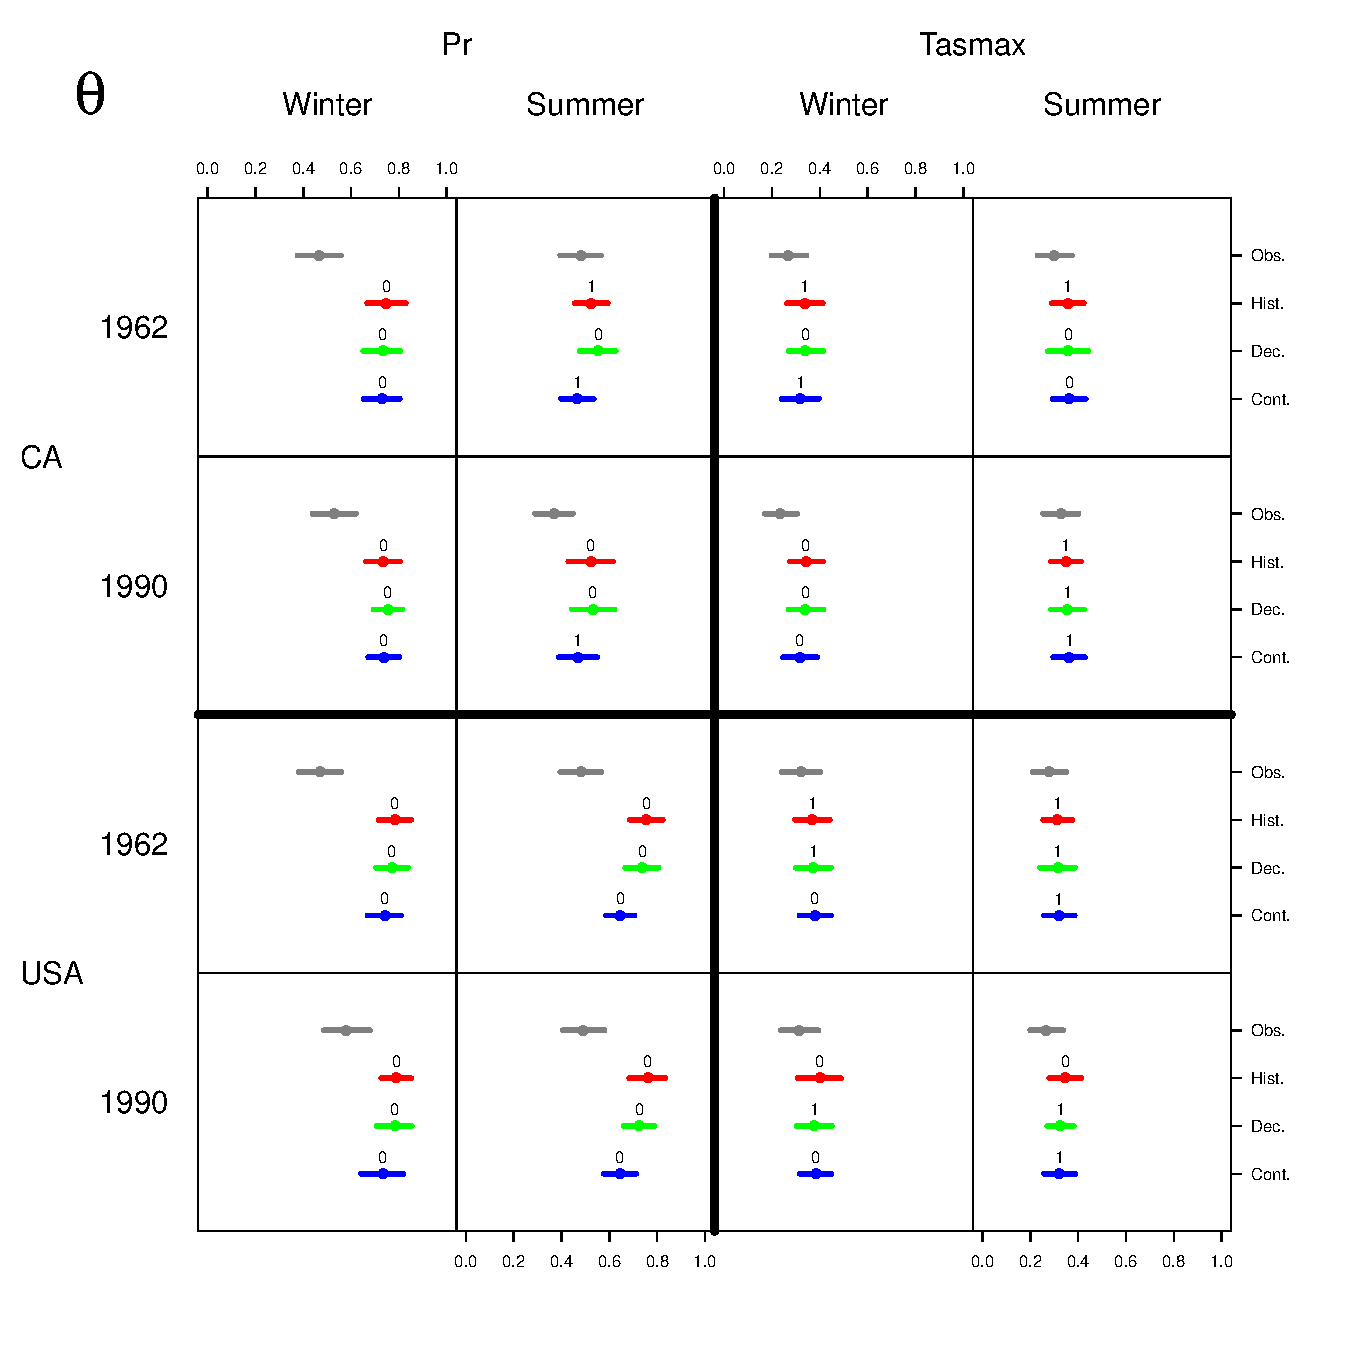
\includegraphics[scale=0.72]{figs/theta.pdf}
\end{center}
\caption{The mean extremal index. Like the parameters shown in Figures \ref{ksi} and \ref{sigma}, the hierarchical mean is shown for the CanCM4 simulations.}
\label{theta}
\end{figure}


Figures \ref{ksi} through \ref{theta} show posterior parameters and other quantities of interest. For the hierarchical model, we show the results of the \emph{mean} process. For example, in Figure \ref{ksi} the parameter shown is the posterior for $\xi$, the mean of $\xi_1,\ldots,\xi_R$. This is in opposition to inference on an unknown replicate which would require sampling, among other things, a new shape parameter $\xi^*$. Therefore, the intervals are more narrow than if we looked at the posterior predictive distribution for a new replicate, but the parameters will be comparable to those from the univariate model with the observations and give us a sense of how the climate simulation performs on average.

The posterior shape parameters in Figure \ref{ksi} show overlapping bounds in many cases, but in some combinations of factors we can see some departure from the observations. The numbers shown above the lines are indicators for whether the posterior from the observations is similar to the posterior of the replicates---in the sense of Bhattacharyya distance described in section \ref{bhatta}---for a particular simulation class.
% TODO: find references for this claim, Weller et al. doesn't confirm it
% Perhaps an unexpected result is that, except for summer precipitation, there is evidence that total precipitation is bounded above (due to $\xi<0$). This is contrary to some findings that the shape parameter for precipitation is positive. [ADD REFS: This was mentioned a lot at SAMSI, so there should be some reference to it, right?]

Figure \ref{sigma} shows the logarithm of the mean scale parameter, $\log(\sigma)$ for the observations and $\log(\alpha/\beta)$ for the simulations, and the posteriors for $\zeta$, the probability of exceeding the threshold, are given in Figure \ref{zeta}.

Figures \ref{20rl} and \ref{50rl} give the $20$- and $50$-year return levels, respectively. In these figures, we have the same $x$-axes for the columns in total precipiation and for the columns under average maximum temperature. Some intervals are difficult to see given the scale, but we can still inspect how the return levels from the observations differ from those of the climate siulations. There is evidence of similarity between the data sources for maximum temperature (except for the 1962--1971 decade in the United States). The simulations struggle to find agreement with the observations when considering precipitation, only having two domains where the observations are similar to at least two of the climate sources (1990 USA Winter and 1962 USA Summer).

Figure \ref{tail} shows posterior predictive samples (based on the mean parameters for the hierarchical model) drawn from the generalized Pareto distribution, conditioned on the random variables being greater than the given threshold. With respect to the 95\% posterior intervals, there is significant overlap of the simulations with the observations, but this is not the case with Bhattacharyya distance. This is because nearly all replicates were very close to their mean, having a distance of roughly $0.02$, while the observations were different enough to have a distance of about $0.2$ from the mean process. Despite all this, we saw in Figures \ref{20rl} and \ref{50rl} that there is still some similarity between the important return level quantities, which account for $\zeta$ and $\theta$.

The posterior mean and 95\% highest posterior density intervals for the extremal index are shown in Figure \ref{theta}. The climate simulations seem to be consistent with the observations for the temperature, but not so for precipiation where they tend to overestimate $\theta$. The Bhattacharyya distance was not computed for these parameters.

\section{Discussion}
\label{discussion}

We have proposed a hierarchical threshold model to handle replicates of climate simulations. The model was applied to a variety of factor combinations and compared to a univariate threshold model for observations. A handful of similarities and differences were found to exist between simulations and the observation product.

We have accounted for trends in the time-series by subtracting out the mean of dynamic linear models, thus yielding anomalies. This poses issues of interpretability and practicality. Our extreme value analysis are in terms of the anomalies and this may not be terribly useful when making comparisons. Should we be interested in the precipitation or temperature extremes in real terms, we must add back the (possibly unknown) mean. However, with a sufficient model on the mean, it would not be unreasonable to use our analysis for projecting extremes in the future.

Some improvement on our use of the Bhattacharyya distance can be made. In this paper we decided that the observations were ``similar'' enough to the climate simulations if the Bhattacharyya distance fell within the distances from the replicates to their mean. A better approach may be to compute a bootstrap sample of the distances and then calculate the proportion of times this exceeds the distance from the observations. 

The next step is to perform a bivariate analysis, with a vision toward the multivariate setting. This bivarate analysis is complicated due to there being replicates in the climate simulations as well as a large variety of factor combinations at which to make the comparisons.


\bibliography{refs}
\bibliographystyle{asa}

\end{document}
